% #######################################
% ########### FILL THESE IN #############
% #######################################
\def\mytitle{MATRICES}
\def\mykeywords{}
\def\myauthor{GOWTHAMI MANDAVA}
\def\contact{gowthamimandava999@gmail.com}
\def\mymodule{ Future Wireless Communication(FWC22012)}
% #######################################
% #### YOU DON'T NEED TO TOUCH BELOW ####
% #######################################
\newcommand{\myvec}[1]{\ensuremath{\begin{pmatrix}#1\end{pmatrix}}}
\let\vec\mathbf
\providecommand{\pr}[1]{\ensuremath{\Pr\left(#1\right)}}
\providecommand{\qfunc}[1]{\ensuremath{Q\left(#1\right)}}
\providecommand{\sbrak}[1]{\ensuremath{{}\left[#1\right]}}
\providecommand{\lsbrak}[1]{\ensuremath{{}\left[#1\right.}}
\providecommand{\rsbrak}[1]{\ensuremath{{}\left.#1\right]}}
\providecommand{\brak}[1]{\ensuremath{\left(#1\right)}}
\providecommand{\lbrak}[1]{\ensuremath{\left(#1\right.}}
\providecommand{\rbrak}[1]{\ensuremath{\left.#1\right)}}
\providecommand{\cbrak}[1]{\ensuremath{\left\{#1\right\}}}
\providecommand{\lcbrak}[1]{\ensuremath{\left\{#1\right.}}
\providecommand{\rcbrak}[1]{\ensuremath{\left.#1\right\}}}
\documentclass[10pt, a4paper]{article}
\usepackage[a4paper,outer=1.5cm,inner=1.5cm,top=1.75cm,bottom=1.5cm]{geometry}
\twocolumn
\usepackage{circuitikz}
\usepackage{amsmath,bm}
\usepackage{amsthm}
\usepackage{mathtools}
\usepackage{amsfonts}
\usepackage{amssymb}
\usepackage{graphicx}
\graphicspath{{./images/}}
%colour our links, remove weird boxes
\usepackage[colorlinks,linkcolor={black},citecolor={blue!80!black},urlcolor={blue!80!black}]{hyperref}
%Stop indentation on new paragraphs
\usepackage[parfill]{parskip}
%% Arial-like font
\usepackage{lmodern}
\renewcommand*\familydefault{\sfdefault}
%Napier logo top right
\usepackage{watermark}
%Lorem Ipusm dolor please don't leave any in you final report ;)
\usepackage{karnaugh-map} 
\usepackage{tabularx}
\usepackage{lipsum}
\usepackage{xcolor}
\usepackage{listings}
%give us the Capital H that we all know and love
\usepackage{float}
%tone down the line spacing after section titles
\usepackage{titlesec}
%Cool maths printing
\usepackage{amsmath}
%PseudoCode
\usepackage{algorithm2e}

\titlespacing{\subsection}{0pt}{\parskip}{-3pt}
\titlespacing{\subsubsection}{0pt}{\parskip}{-\parskip}
\titlespacing{\paragraph}{0pt}{\parskip}{\parskip}
\newcommand{\figuremacro}[5]{
    \begin{figure}[#1]
        \centering
        \includegraphics[width=#5\columnwidth]{#2}
        \caption[#3]{\textbf{#3}#4}
        \label{fig:#2}
    \end{figure}
}


 \lstset{
frame=single, 
breaklines=true,
columns=fullflexible
}

\thiswatermark{\centering \put(1,-110){
\includegraphics[scale=0.05]{IIT_logo.jpg}} }
\title{\mytitle}
\author{\myauthor\hspace{1em}\\\contact\\IITH\hspace{0.5em}-\hspace{0.5em}\mymodule}
\date{}
\hypersetup{pdfauthor=\myauthor,pdftitle=\mytitle,pdfkeywords=\mykeywords}
\sloppy
% #######################################
% ########### START FROM HERE ###########
% #######################################
\begin{document}
 \maketitle
 \tableofcontents
  \Large\section{Problem}
 \textbf{Q}.
 \begin{equation}
	x^2+4y^2=4
	\end{equation}is the equation of ellipse which is inscribed in a rectangular aligned with the co-ordinate axes,which is turn is inscibed in another ellipse that passes through the point (4,0).Then the equation of ellipse
 \section{Solution}
 \begin{center}
     Given,
      the equation of ellipse is \begin{equation}
      x^2+4y^2=4 
      \end{equation}
      \\ and point passing through another ellipse \textbf{Q}=\myvec{4\\0}
      \begin{equation}
       x^2/4+y^2=1  
       \end{equation}
       \begin{equation}
       {\lambda}_{1}=1/4 
       {\lambda}_{2}=1
      \end{equation}
      \\ hence a=2 and b=1
       \\ the standard equation of ellipse using matrices can be written as,
       \begin{align}
    \\\textbf{x}^{\top}\textbf{V}\textbf{x}=1
    \end{align}
      where 
      \begin{equation}
      \textbf{V}=\myvec{\lambda1 & 0 \\ 0 & \lambda2} 
      \end{equation}
      \begin{equation}
      \textbf{V}=\myvec{1/4 & 0 \\ 0 & 1}
      \end{equation}
      \begin{equation}
      \textbf{x}^{\top}\myvec{1/4 & 0 \\ 0 & 1}\textbf{x}=1
      \end{equation}
      the equation of tangents that passing through \textbf{l}=\myvec{a,0} and \textbf{m}=\myvec{0,b} is 
      \begin{align}
  (\textbf{V}\textbf{l}+\textbf{u})^{\top}\textbf{X}+\textbf{u}^{\top}\textbf{l}+f=0
  \\ (\textbf{V}\textbf{m}+\textbf{u})^{\top}\textbf{X}+\textbf{u}^{\top}\textbf{m}+f=0
   \end{align}
   as \textbf{u}=\myvec{0\\0} and f=-1 we get
   \begin{equation}
    \myvec{(\textbf{V}\textbf{l})^{\top} \\ (\textbf{V}\textbf{m})^{\top}}\textbf{X}=\myvec{1\\1}
   \end{equation}  
   by solving them we get
   \begin{align*}
   \myvec{1/2&0&1\\0&1&1}  \xrightarrow[]{R_1 \leftarrow R_1*2 }
   \\ \myvec{1&0&2\\0&1&1}
\end{align*}        
point of intersection of two tangents is \textbf{P}=\myvec{2\\1}
\\ from the given information  \textbf{p} touches the second ellipse and \textbf{Q} is also passing through it.so we can write the equaion od ellipse as
 \begin{align} 
 \textbf{P}^{\top}\textbf{V}\textbf{P}=1
         \\  \textbf{Q}^{\top}\textbf{V}\textbf{Q}=1 
        \end{align}
              
        we can write them as
       \begin{align} 
          \textbf{P}^{\top}\textbf{v}\textbf{p}=1
          \\ \textbf{Q}^{\top}\textbf{v}\textbf{q}=1 
          \end{align}
          as
          \begin{equation}
          \textbf{v}=\myvec{{\lambda}_{1}\\{\lambda}_{2}}
          \; \textbf{p}=\myvec{2&0\\0&1} 
         \; \textbf{q}=\myvec{4&0\\0&0}
          \end{equation}
          the matrix form of above equations is
          \begin{align} 
            \myvec{\textbf{P}^{\top}\textbf{p} \\ \textbf{Q}^{\top}\textbf{q}}\textbf{v}=1
           \end{align}
             \\  substituting appropriate values we get
             \begin{align}
              \\\myvec{4&1\\16&0}\textbf{v}=\myvec{1\\1}
\end{align}
\end{center}
solving the above equation
\begin{center}            
\begin{align}       
\myvec{4&1&1 \\16&0&1} \xrightarrow[]{R_1 \leftarrow R_1/4 } 
\end{align}
\begin{align}
\myvec{1 & 1/4 & 1/4 \\16 & 0 & 1} \xrightarrow[]{R_2 \leftarrow -16R_1+R_2 } 
\end{align}
\begin{align}
\myvec{1 & 1/4 & 1/4 \\0&-4&-3} \xrightarrow[]{R_2 \leftarrow  R_2/-4 }
\end{align}
\begin{align}
\myvec{1&1/4&1/4 \\0 & 1 & 3/4 } \xrightarrow[]{R_1 \leftarrow R_1- R_2/4 }
\end{align}
\begin{align}
\myvec{1&0&1/16 \\0 & 1 & 3/4  }
\end{align} 
\end{center}
By solving the above equations we get \\ 
\begin{equation}
{\lambda}_{1}=1/16\ and\; {\lambda}_{2}=3/4
\end{equation}
the required equation of ellipse is 
\begin{equation}
\textbf{x}^{\top}\myvec{1/16&0\\0&3/4}\textbf{x}=1    
\end{equation} 
we get \begin{equation}
x^2/16+3y^2/4=1 
\end{equation}
 \section{Plot}
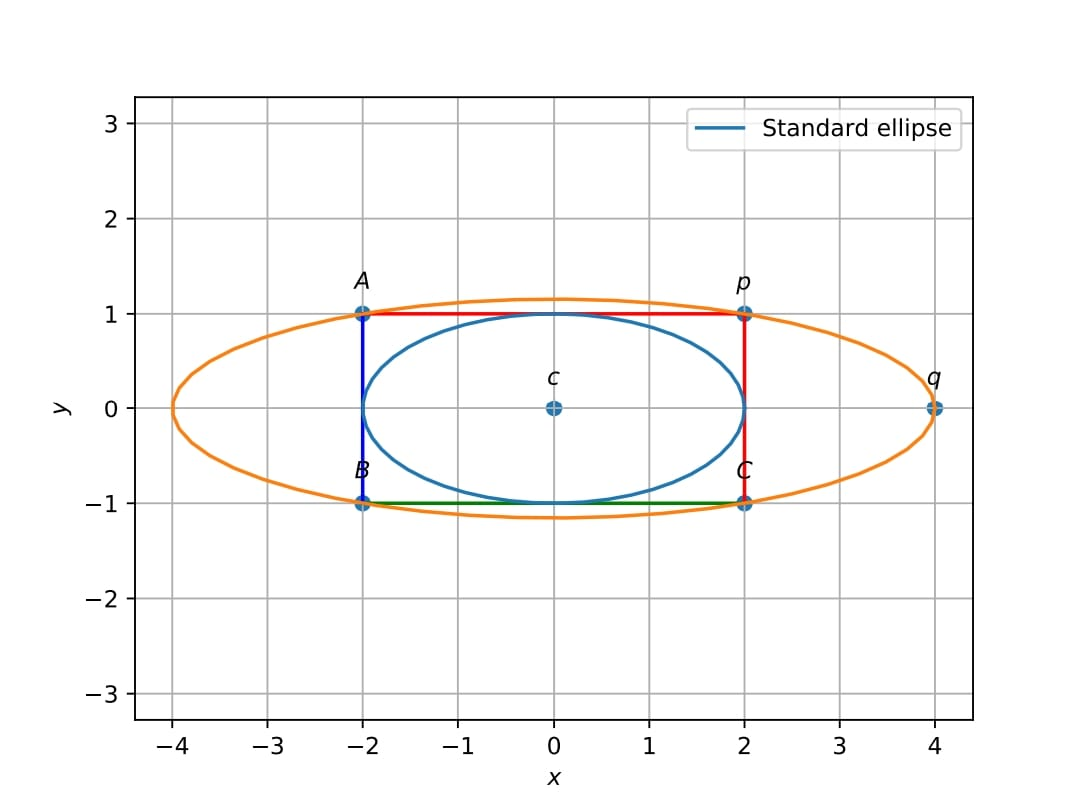
\includegraphics[scale=0.25]{ellipse.jpg}
  \section{Software}
  We can plot the cicle with the help of the following code :
 \vspace{3mm} 
\begin{lstlisting}
https://github.com/Gowt-hami/fwc-1-module1/blob/main/par.py
\end{lstlisting}
\end{document}
